\section{Software}

\subsection{Measurement Setup}

The validation of the software was done using the \lstcpp{Tabel} class. This class provides multiple vectors which can be used to save samples or other data. When the program is exited this data is written to stdout using the \textit{CSV} format. This can then be analyzed directly in the terminal or printed to a file and imported into a python notebook.\p
%
Instead of sending the resulting signal over SPI a timestamp is generated and both (timestamp and signal) are added to the table. Additionally, the duration of one iteration (with sleep) is saved. %Finally the position in the table is increased to the next row with \lstcpp{nexSignal()}.

\subsection{Discussion}

Figure \ref{fig:meas:software:duration} shows the duration of each iteration over the transmission of a $1\,s$ signal. It can be observed that the loop does not reach a stable duration. The smaller variations can be explained by the scheduling of Linux and should not be a problem. However the graph also shows larger deviations from the intended $10\,\mu s$ loop duration wich could have an impact on the quality of the output signal.
%
\begin{figure}[ht]
  \centering
  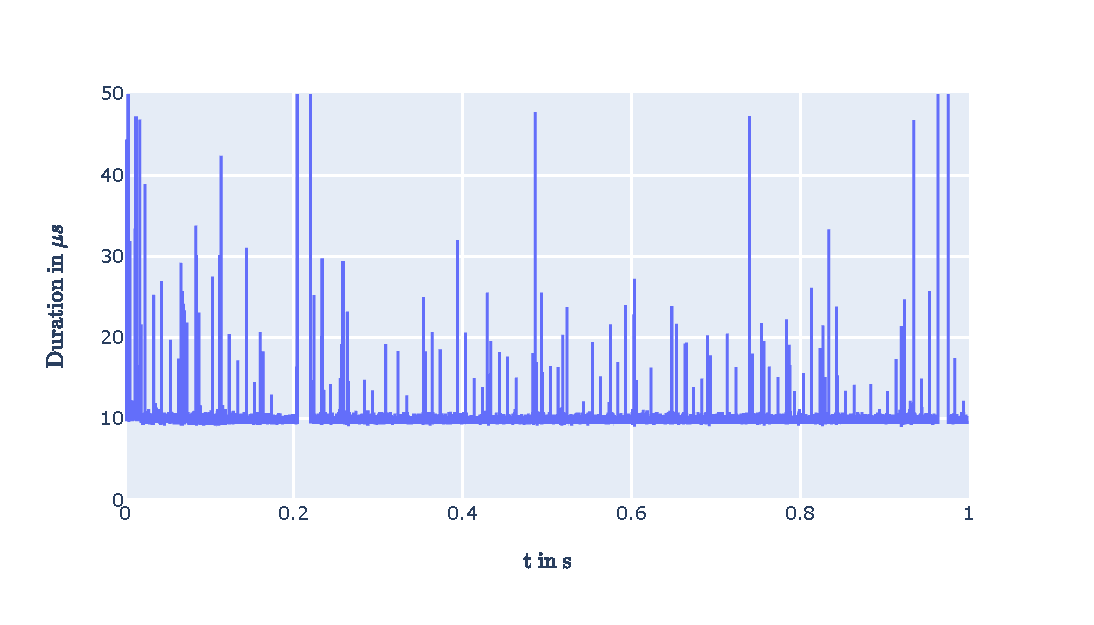
\includegraphics[height=\mediumheight]{src/assets/pictures/measurements/software_duration.pdf}
  \caption{Duration of the loop}\label{fig:meas:software:duration}
\end{figure}
\newpage\noindent
In Figure \ref{fig:meas:software:am} the time and frequency spectrum of an amplitude modulated sine wave generated by the sound laser software is displayed. The time plot shows a clearly recognizable AM signal while the frequency spectrum is quite distorted. However the peak of the carrier wave as well as the upper and lower sideband are unmistakable.
%
\begin{figure}
  \centering
  \begin{subfigure}[b]{0.8\textwidth}
    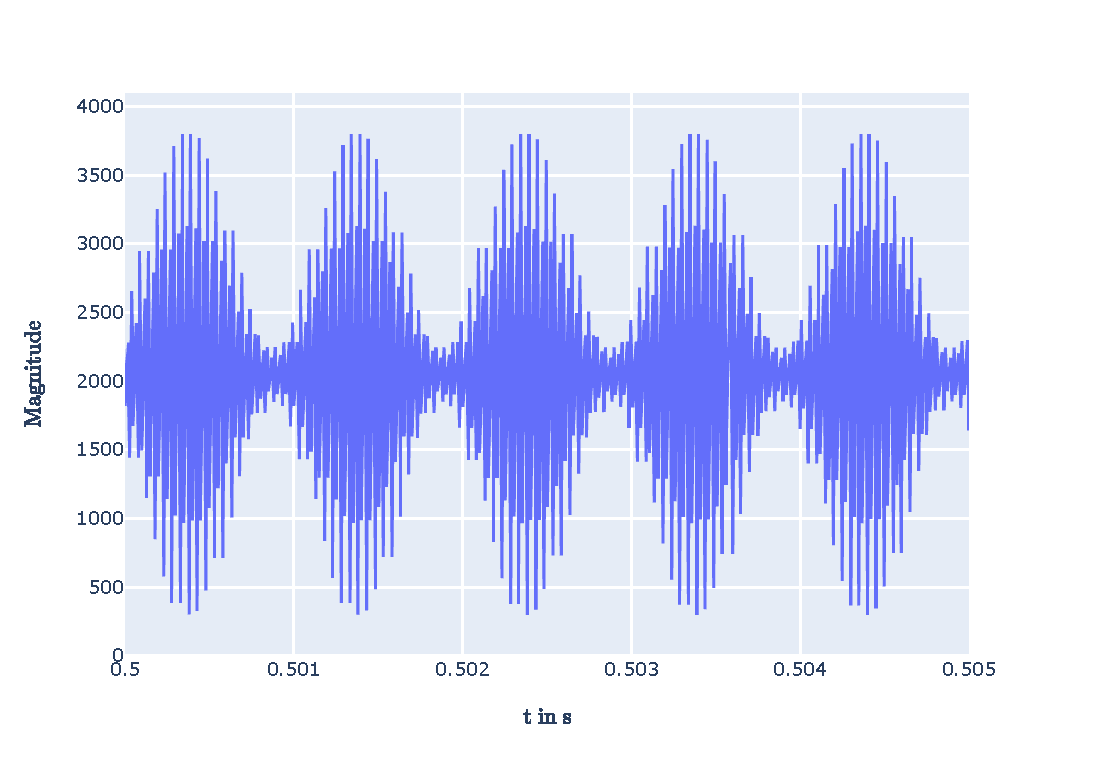
\includegraphics[width=\textwidth]{src/assets/pictures/measurements/software_am_time.pdf}
    \caption{Time signal}
    \label{fig:meas:software:am_time}
  \end{subfigure}
  \hfill
  \begin{subfigure}[b]{0.8\textwidth}
    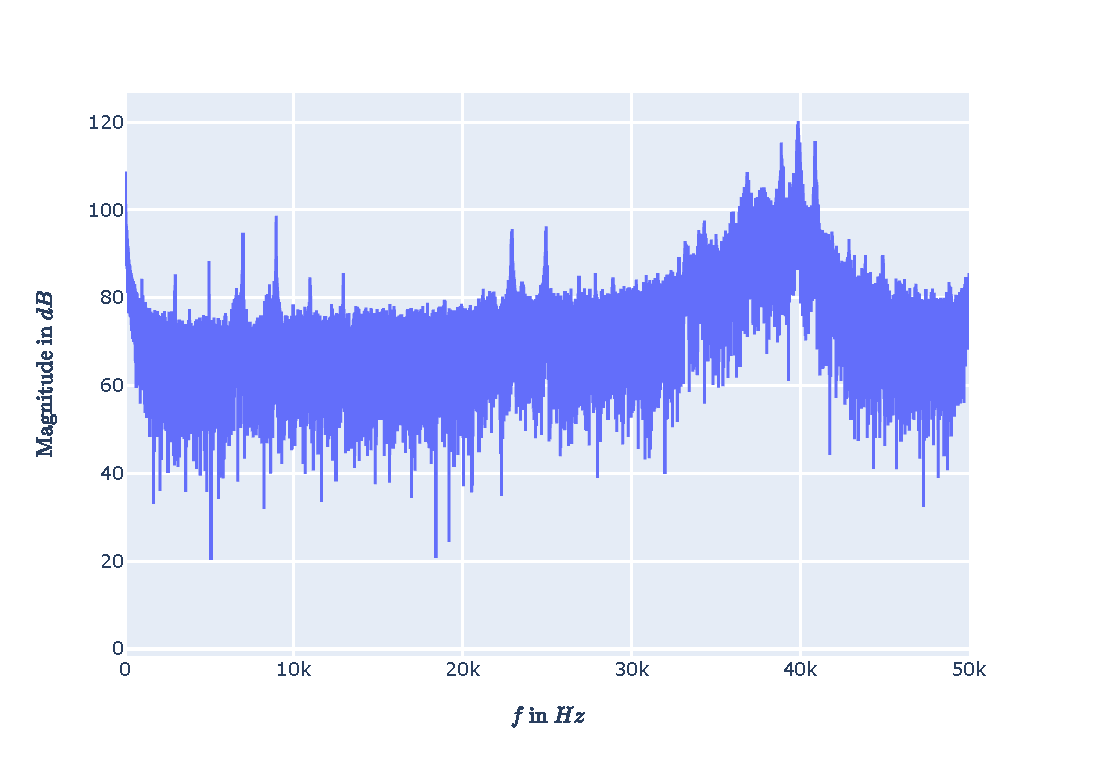
\includegraphics[width=\textwidth]{src/assets/pictures/measurements/software_am_frequency.pdf}
    \caption{Frequency spectrum}
    \label{fig:meas:software:am_freq}
  \end{subfigure}
  \caption{AM modulated sine wave}
  \label{fig:meas:software:am}
\end{figure}
%
\subsection{Audiotest}

In addition to the measurements above the software was tested by listening to it using the speaker module. Because the original DAC did not work (See section \secref{sec:meas:circuit:dac}) an 8 Bit DAC (MCP4901T) was used. Different sine waves as well as a song where played. In the resulting audio all sounds could be recognized. Unfortunately, the signal was very noisy. As analyzed before in figure \ref{fig:meas:software:duration} the signal also paused repeatedly for a short time.